%% AMS-LaTeX Created with the Wolfram Language : www.wolfram.com

\documentclass[12pt]{article}
\usepackage{ceai} % Style file is in the project root.
\graphicspath{{../figs/}}

\begin{document}
\doublespacing	

\title{CE 488/5588: Applied Artificial Intelligence\\ \large Topic 12: Classic Unsupervised Learning}
\author{}
\date{}
\maketitle

\section{Introduction}

Having covered supervised discriminative learning, supervised generative learning, and supervised regression in the previous topics, we now turn to the other major paradigm of machine learning: \textbf{unsupervised learning}. In this setting, the data are given without class labels or regression targets. The objective is therefore not to predict a known output, but to uncover structure already present in the data.

Given a dataset
\[
 \mathcal{D} = \{ \bm{x}_n \mid n = 1, 2, \cdots, N\}
\]
where each data point $\bm{x}_n\in \mathbb{R}^d$. Compared with the datasets used in supervised learning, there are now no labels attached to the samples. This changes the role of learning significantly. Instead of fitting a decision boundary or a regression function, we seek patterns such as groups, low-dimensional structure, redundancy, or abnormal behavior.

Two classical tasks dominate this topic. The first is \textbf{clustering}, in which similar samples are grouped together according to their geometry in feature space. The second is \textbf{dimensionality reduction}, in which the original variables are replaced by a smaller number of informative coordinates while preserving essential structure. In engineering applications, these tools are useful for exploratory analysis, operating-regime identification, anomaly screening, visualization, denoising, and preprocessing before later supervised learning.

After this topic, you should be able to:

\begin{itemize}
    \item explain the role of unsupervised learning and distinguish clustering from dimensionality reduction;
    \item formulate the objective of k-means clustering and explain how the algorithm iteratively improves a partition;
    \item describe how hierarchical clustering and DBSCAN differ from k-means in assumptions, outputs, and practical behavior;
    \item evaluate clustering results using internal and external criteria; and
    \item explain how PCA constructs a low-dimensional representation and why nonlinear dimensionality-reduction methods may also be useful.
\end{itemize}


\section{Clustering}
Clustering groups samples so that points within the same cluster are relatively similar while points from different clusters are relatively dissimilar. Because no labels are given, the meaning of a cluster is not known in advance; it must be inferred from the structure of the data and then interpreted in context. Different clustering algorithms define similarity differently, so method selection should reflect the expected geometry of the dataset.

\subsection{K-means clustering}

K-means is a prototype-based clustering method that partitions a dataset 
\[
\mathcal{D} = \{ \bm{x}_n \mid n=1,2,\ldots,N\}, \quad \bm{x}_n \in \mathbb{R}^d,
\]
into $K$ clusters by minimizing the sum of squared distances between each sample and its assigned cluster centroid. Its objective function is
\begin{equation}
J = \sum_{k=1}^{K} \sum_{\bm{x}_i \in S_k} \lVert \bm{x}_i - \bm{\mu}_k \rVert^2,
\end{equation}
where $\bm{\mu}_k$ is the centroid of cluster $k$, and $S_k$ is the set of points assigned to that cluster. 

The quantity $J$ is the within-cluster sum of squares. A small value of $J$ indicates that points lie close to the representative centroid of their cluster. The algorithm alternates between two simple operations:
\begin{enumerate}
    \item \textbf{Assignment step:} assign each point to its closest centroid.
    \item \textbf{Update step:} recompute each centroid as the sample mean of the points currently assigned to it.
\end{enumerate}
These two steps are repeated until the assignments stabilize or the decrease in $J$ becomes negligible. Each iteration does not increase the objective, so k-means converges in a finite number of iterations to a local minimum.

\subsubsection{History and Significance}

K-means has deep roots in pattern recognition and vector quantization:
\begin{itemize}
    \item \textbf{Early Formulations:} Variants of the algorithm appeared in the 1950s and 1960s. It was formalized by James MacQueen in 1967 and later popularized by Stuart Lloyd in 1980 (commonly known as Lloyd’s algorithm).
    \item \textbf{Simplicity and Efficiency:} The method's straightforward iterative process, assigning points to the nearest centroid and then updating centroids based on the cluster means, makes it easy to understand.
    \item \textbf{Wide Applicability:} K-means has been successfully applied in diverse areas, such as image segmentation, market segmentation, document clustering, and bioinformatics, making it a baseline method for many clustering tasks.
\end{itemize}


\subsubsection{Expectation-Maximization (EM) Algorithm}
The Expectation-Maximization (EM) algorithm is a general iterative framework for problems that involve hidden or latent variables. It alternates between estimating latent quantities and updating model parameters. K-means can be interpreted as a special, hard-assignment version of this broader idea.


K-means can be viewed as a special case of the EM algorithm with hard assignments:
\begin{enumerate}
    \item \textbf{E-step (Assignment):} For each data point $\bm{x}_n$, assign it to the closest centroid:
    \begin{equation}
    S_k = \{ i : \lVert \bm{x}_i - \bm{\mu}_k \rVert \leq \lVert \bm{x}_i - \bm{\mu}_j \rVert,\ \forall\, j \neq k \}
    \end{equation}
    \item \textbf{M-step (Update):} Update each centroid by minimizing the objective function with respect to $\bm{\mu}_i$, which is achieved by computing the sample mean:
    \begin{equation}
    \bm{\mu}_k = \frac{1}{|S_k|} \sum_{i \in S_k} \bm{x}_i
    \end{equation}
\end{enumerate}
Each iteration decreases the objective function $J$ because:
\begin{itemize}
    \item The E-step minimizes $J$ by assigning each data point to the closest centroid.
    \item The M-step minimizes $J$ with respect to $\bm{\mu}_k$, as the sample mean is the least-squares estimator.
\end{itemize}
This interpretation is useful because it connects a geometrically intuitive algorithm to a more general statistical optimization principle. It also explains why initialization matters: different starting centroids may lead to different local minima.

\subsubsection{Computational Considerations}

Several factors influence the performance of k-means in practice:
\begin{itemize}
    \item \textbf{Distance Metric:} K-means conventionally employs the Euclidean distance:
    \[
    \lVert \bm{x}_i - \bm{\mu}_k \rVert^2,
    \]
    which aligns with the objective function. Alternative metrics may be used for specific applications but require adaptations in the algorithm’s theoretical framework.
    \item \textbf{Convergence Criteria:} The algorithm is typically terminated when:
    \begin{itemize}
        \item \textit{Centroid Stability:} The relative change in centroid positions is below a threshold $\epsilon$:
        \[
        \frac{\lVert \bm{\mu}_k^{(t+1)} - \bm{\mu}_k^{(t)} \rVert}{\lVert \bm{\mu}_k^{(t)} \rVert} < \epsilon \quad \forall\, k.
        \]
        \item \textit{Objective Function Change:} The decrease in $J$ between iterations is negligible:
        \[
        \frac{|J^{(t+1)} - J^{(t)}|}{J^{(t)}} < \epsilon.
        \]
    \end{itemize}
    \item \textbf{Feature scaling:} Since the assignments are driven by distances, features with larger numerical ranges can dominate the clustering unless the data are standardized or normalized.
    \item \textbf{High-dimensionality:} Each iteration’s computational cost is approximately
    \[
    \mathcal{O}(N \times K \times d),
    \]
    where $d$ is the dimensionality. In high-dimensional spaces, not only does the computation become more intensive, but the Euclidean distance can lose discriminative power, often necessitating the use of dimensionality reduction techniques (e.g., PCA) prior to clustering.
\end{itemize}

\subsubsection{Determining the Number of Clusters}

Choosing the number of clusters $K$ is a classical challenge in k-means clustering. Figure~\ref{fig:topic12-kmeans-k3-k5} first gives a visual reminder of why this choice matters. When $K=3$, the recovered partition matches the three dominant groups in the dataset reasonably well; when a larger value such as $K=5$ is forced, k-means tends to split natural groups into smaller pieces. This visual effect motivates a more systematic way to select $K$.

\begin{figure}[t]
    \centering
    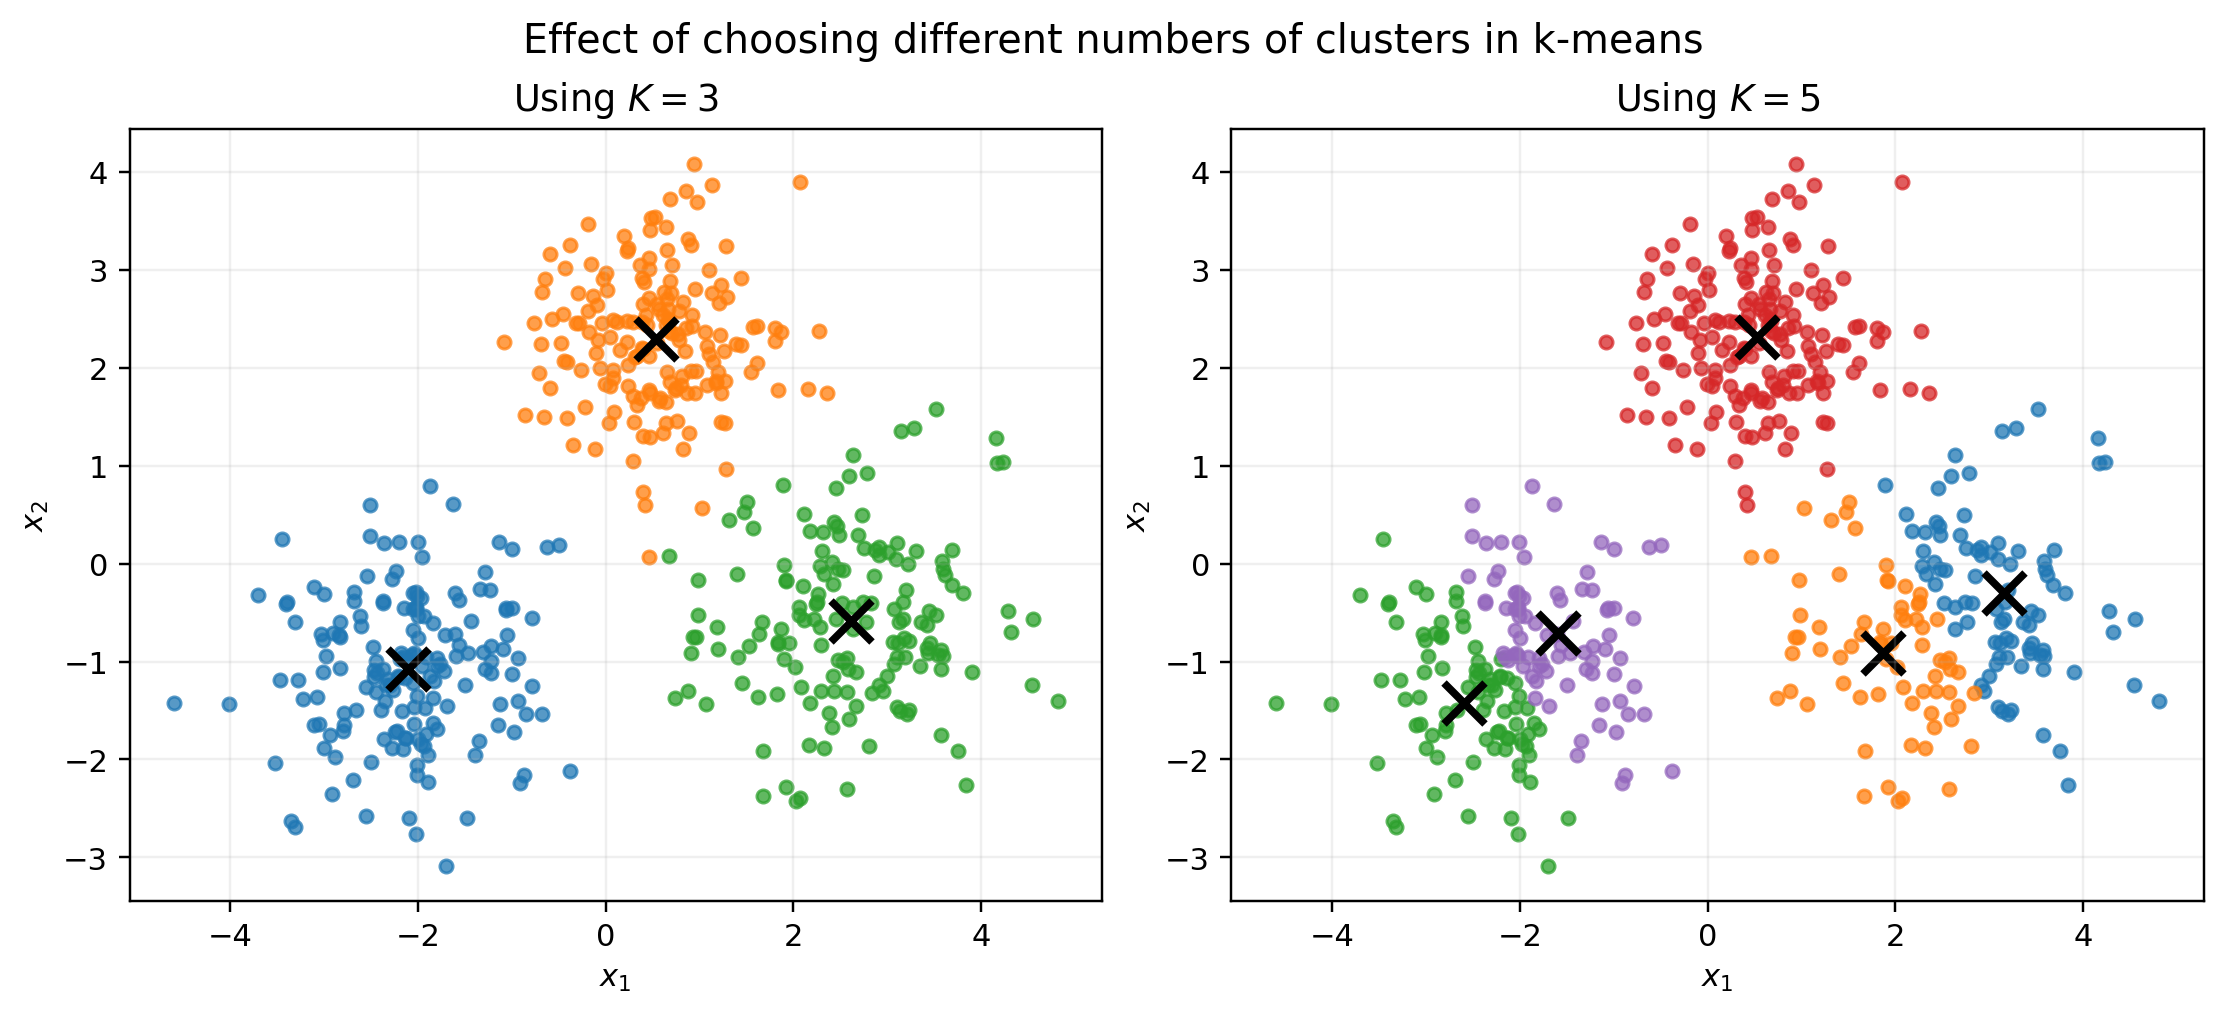
\includegraphics[width=0.92\textwidth]{topic12_kmeans_k3_vs_k5.png}
    \caption{Visual effect of choosing different values of $K$ in k-means on the same dataset. The left panel uses $K=3$, while the right panel uses a larger value, $K=5$, which produces a finer partition. Figure generated for this chapter using a synthetic dataset in the style of standard k-means demonstrations.}
    \label{fig:topic12-kmeans-k3-k5}
\end{figure}

Common methods include:
\begin{itemize}
    \item \textbf{Elbow Method:} Plot the objective function $J$ versus $K$ and identify the point where the reduction in $J$ begins to plateau ("elbow"), suggesting that additional clusters provide diminishing returns.
    \item \textbf{Silhouette Analysis:} Compute the silhouette coefficient,
    \[
    s(\bm{x}_n) = \frac{b(\bm{x}_n) - a(\bm{x}_n)}{\max\{a(\bm{x}_n), b(\bm{x}_n)\}},
    \]
    where $a(\bm{x}_n)$ is the average distance to points in the same cluster and $b(\bm{x}_n)$ is the minimum average distance to points in another cluster. A higher average silhouette score indicates a better clustering structure.
    % \item \textbf{Information Criterion Methods:} When k-means is seen as a limiting case of a Gaussian Mixture Model, criteria such as the Bayesian Information Criterion (BIC) or Akaike Information Criterion (AIC) can help balance model fit and complexity.
\end{itemize}
% These methods provide insights into the trade-offs of different choices of $K$, and in practice, a combination of approaches is often used.
Figure~\ref{fig:topic12-elbow} then shows the corresponding elbow-style plot used for this model-selection step.

\begin{figure}[t]
    \centering
    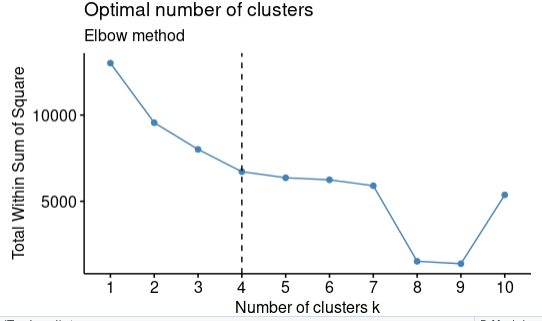
\includegraphics[width=0.5\textwidth]{topic12_elbow_method.png}
    \caption{An example of the elbow method for selecting the number of clusters in k-means. Courtesy of Wikimedia Commons (\texttt{Elbow\_method.png}).}
    \label{fig:topic12-elbow}
\end{figure}


\subsection{Hierarchical clustering}

Hierarchical clustering builds a nested sequence of clusters rather than directly producing one partition for a prescribed value of $K$. In the agglomerative version, which is the most common, the algorithm begins with each sample as its own cluster and repeatedly merges the two closest clusters. The output is a tree structure called a \textbf{dendrogram}.

An important modeling choice is the distance between two clusters. Common linkage rules include:
\begin{itemize}
    \item \textbf{single linkage:} distance between the closest pair of points;
    \item \textbf{complete linkage:} distance between the farthest pair of points;
    \item \textbf{average linkage:} average pairwise distance; and
    \item \textbf{Ward linkage:} increase in within-cluster variance after merging.
\end{itemize}
One advantage of hierarchical clustering is that it does not require the user to fix the number of clusters in advance. Instead, one may inspect the dendrogram and choose a cut level that yields a desired grouping resolution. This is useful when the data may exhibit meaningful structure at multiple scales. Figure~\ref{fig:topic12-dendrogram} illustrates this nested view of merging. Its main limitations are computational cost on large datasets and sensitivity to the chosen linkage and distance metric.

\begin{figure}[t]
    \centering
    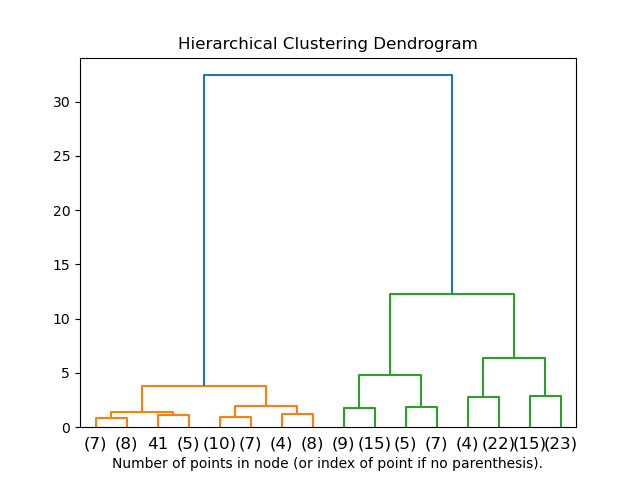
\includegraphics[width=0.55\textwidth]{topic12_hierarchical_dendrogram.png}
    \caption{A dendrogram visualizes the sequence of agglomerative merges in hierarchical clustering. Courtesy of the scikit-learn hierarchical clustering example.}
    \label{fig:topic12-dendrogram}
\end{figure}

\subsection{DBSCAN}
DBSCAN (Density-Based Spatial Clustering of Applications with Noise) is a density-based clustering method that groups data points that are closely packed while explicitly identifying isolated samples as noise. It can find clusters of arbitrary shape and does not require the number of clusters to be specified in advance.

Given a radius parameter $\epsilon$, the $\epsilon$-neighborhood of a point $\bm{x}_n$ is
\[
\mathcal{N}_{\epsilon}(\bm{x}_n) = \{\bm{x}_j \in \mathcal{D} \mid \|\bm{x}_j-\bm{x}_n\| \leq \epsilon\}.
\]
If this neighborhood contains at least \textit{MinPts} samples, then $\bm{x}_n$ is called a \textbf{core point}. Clusters are formed by connecting core points that are density-reachable from one another. Points close to a cluster but not dense enough to be core points are often called border points, while isolated points are labeled as noise.

DBSCAN is especially attractive when clusters are nonconvex or when outlier detection is important. Its main weakness is parameter sensitivity: if $\epsilon$ is too small, many points are labeled as noise; if it is too large, distinct clusters may merge. Figure~\ref{fig:topic12-dbscan} shows the type of irregular cluster geometry that motivates density-based methods. Like other distance-based methods, it also becomes more difficult in very high-dimensional spaces.

\begin{figure}[t]
    \centering
    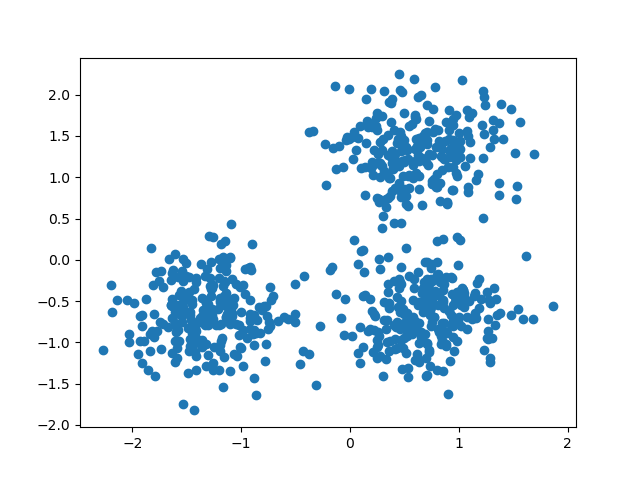
\includegraphics[width=0.55\textwidth]{topic12_dbscan.png}
    \caption{DBSCAN can recover dense clusters of irregular shape while identifying noise points. Courtesy of the scikit-learn DBSCAN example.}
    \label{fig:topic12-dbscan}
\end{figure}

\section{Clustering Evaluation}
Performance evaluation in clustering is different from performance evaluation in supervised classification. Since true labels are usually unavailable, the question is not simply whether a predicted class agrees with a ground-truth class. Instead, we ask whether the clustering is compact, separated, stable, and meaningful for the application. There are two broad categories of evaluation methods: internal and external evaluation.

\subsection{Internal evaluation}
 Internal evaluation methods assess the quality of the clustering without using any external labels. Some common internal evaluation metrics include:
    \begin{itemize}
      \item \textit{Inertia (Sum of Squared Errors)}: Inertia measures the sum of squared distances between each data point and its assigned cluster centroid. A lower inertia value indicates tighter clusters. Inertia is primarily used for evaluating K-means clustering.
      \item \textit{Silhouette Score}: The silhouette score measures the average intra-cluster cohesion and inter-cluster separation. It ranges from -1 to 1, with a higher score indicating better clustering.
      \item \textit{Calinski-Harabasz Index}: The Calinski-Harabasz index measures the ratio of between-cluster dispersion to within-cluster dispersion. A higher value indicates better clustering.
    \end{itemize}
  These measures are useful for comparing candidate clusterings, choosing hyperparameters, and deciding whether the recovered groups are geometrically meaningful.


\subsection{External evaluation}
External evaluation methods compare the clustering result with some external ground truth or reference information, such as expert annotations or known classes that were not used during clustering. Some common external evaluation metrics include:

    \begin{itemize}
      \item \textit{Adjusted Rand Index (ARI)}: The ARI measures the similarity between two clustering assignments, adjusting for chance. It ranges from -1 to 1, with 1 indicating perfect agreement and 0 indicating the expected agreement by chance.
      \item \textit{Normalized Mutual Information (NMI)}: NMI measures the mutual information between two clustering assignments, normalized by the geometric mean of their individual entropies. It ranges from 0 to 1, with 1 indicating perfect agreement and 0 indicating no shared information.
      \item \textit{Fowlkes-Mallows Index}: The Fowlkes-Mallows index measures the geometric mean of precision and recall, with values ranging from 0 to 1. A higher value indicates better agreement between the clustering and the ground truth.
    \end{itemize}
  External evaluation methods can provide more objective assessments, but they are available only when some trusted reference grouping exists. In practice, numerical indices should still be interpreted together with engineering judgment, because a mathematically compact clustering is not necessarily the most useful one for decision making.

\section{Dimensionality Reduction}

Clustering aims to group samples; dimensionality reduction aims to represent each sample using fewer variables. This is important when the original feature space is high-dimensional, redundant, noisy, or difficult to visualize. A lower-dimensional representation can reveal dominant structure, suppress noise, and sometimes improve the behavior of later learning algorithms.

\subsection{Principal Component Analysis (PCA)}

Principal Component Analysis (PCA) is the classical linear method for reducing dimension. Its goal is to project the data onto a lower-dimensional subspace that preserves as much variance as possible. Let
\[
\bar{\bm{x}} = \frac{1}{N}\sum_{n=1}^{N} \bm{x}_n
\]
be the sample mean. After centering the data, define the covariance matrix
\[
\mathbf{C} = \frac{1}{N}\sum_{n=1}^{N}(\bm{x}_n-\bar{\bm{x}})(\bm{x}_n-\bar{\bm{x}})^T.
\]
PCA chooses orthogonal directions associated with the largest eigenvalues of $\mathbf{C}$. These directions are called the \textbf{principal components}. If $\mathbf{W}_p \in \mathbb{R}^{d\times p}$ collects the first $p$ principal directions, where $p<d$, then the reduced representation of $\bm{x}_n$ is
\[
\bm{y}_n = \mathbf{W}_p^T(\bm{x}_n-\bar{\bm{x}}), \qquad \bm{y}_n \in \mathbb{R}^{p}.
\]
The transformed dataset
\[
\mathcal{Y} = \{\bm{y}_n \mid n=1,2,\ldots,N\}
\]
retains the dominant linear variation of the original data using many fewer coordinates.

PCA is widely used because it is simple, computationally efficient, and interpretable. It is often applied before clustering when features are highly correlated or when Euclidean distances in the original space become less informative. It is also common to inspect the fraction of variance explained by the first few principal components in order to choose a practical reduced dimension. Figure~\ref{fig:topic12-pca} shows how a high-dimensional dataset can be projected into a smaller visualizable space.

\begin{figure}[t]
    \centering
    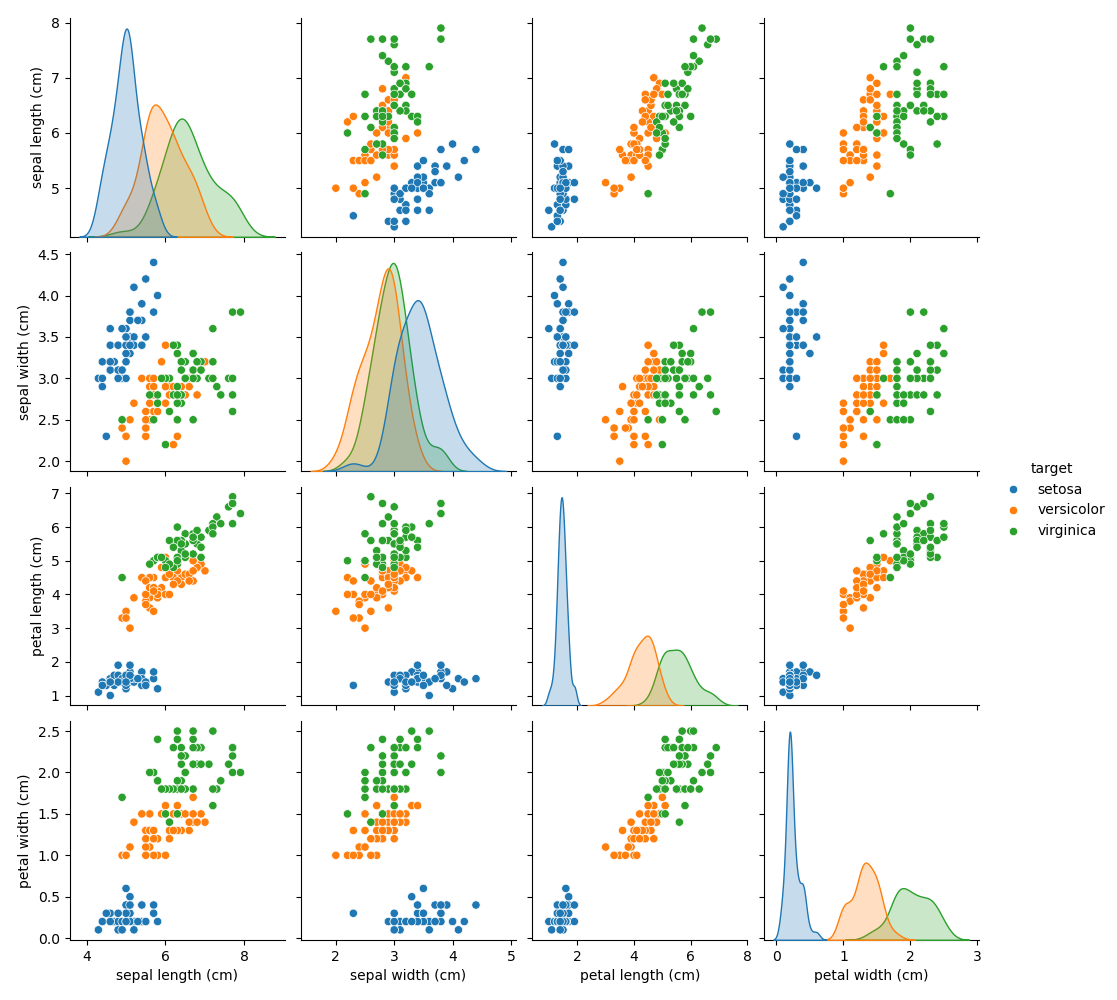
\includegraphics[width=0.65\textwidth]{topic12_pca_iris.png}
    \caption{A PCA projection illustrates how high-dimensional data can be summarized in a smaller number of coordinates for visualization and analysis. Courtesy of the scikit-learn PCA example.}
    \label{fig:topic12-pca}
\end{figure}

\subsection{A Brief Note on Nonlinear Methods}

PCA is a linear method, so it works best when the dominant structure of the data is approximately captured by a flat low-dimensional subspace. This assumption is not always appropriate. In some datasets, the samples lie near a curved manifold in the original feature space, and a linear projection may fail to preserve important neighborhood relationships.

In such cases, nonlinear dimensionality-reduction methods may be useful. Examples include kernel PCA, Isomap, t-SNE, and UMAP. These methods are especially valuable for visualization and exploratory analysis because they can reveal low-dimensional structure that PCA may miss. Their tradeoffs are greater parameter sensitivity, higher computational cost, and usually less direct interpretability. For this reason, PCA remains the natural first choice when the goal is compression, denoising, or stable preprocessing for later engineering models.

\section{Conclusion Remarks}
In this chapter, we examined classical unsupervised learning, where the data are provided without labels or regression targets and the objective is to discover structure directly from the samples themselves. We focused on two major tasks. The first was clustering, studied through k-means, hierarchical clustering, and DBSCAN, which represent centroid-based, tree-based, and density-based views of grouping. The second was dimensionality reduction, where PCA provides a practical linear method for constructing compact representations and nonlinear methods offer additional flexibility when the data geometry is curved.

For engineering applications, the main lesson is that unsupervised learning is not one single algorithm, but a family of tools for organizing, simplifying, and interpreting data before or alongside predictive modeling. Method selection should depend on the geometry of the data, the presence of noise and outliers, the need for interpretability, and the intended downstream use. When applied carefully, clustering and dimensionality reduction can reveal hidden operating regimes, compress high-dimensional measurements, and provide clearer structure for later supervised or unsupervised analysis.

\end{document}
